\documentclass[15pt,a4paper]{report}
% \usepackage[utf8]{inputenc}
% \usepackage[vietnam]{babel}
\usepackage[utf8]{vietnam}
\usepackage{amsmath}
\usepackage{amsfonts}
\usepackage{amssymb}
\usepackage{graphicx}
\usepackage{color}
\usepackage{framed}
\usepackage{cases} 

\usepackage[left=2cm,right=2cm,top=2cm,bottom=2cm]{geometry}

\title{\framebox {
        \textcolor{TEcolor}{
            \Huge {    CALCULUS II    }
        }
    }    }
    
\author{\Large @arch-techs}
\date{2021}

\definecolor{TEcolor}{RGB}{0, 50, 50}

\usepackage{fancyhdr}

\pagestyle{fancy}
\fancyhf{}
\lhead{
\includegraphics[scale=0.2]{TE1}
\textcolor{TEcolor}{
\fontfamily{cmss}\selectfont
@arch-techs}
}
\rhead{\textcolor{TEcolor} {
	\fontfamily{cmss}\selectfont CALCULUS II
}}
\rfoot{
\fontfamily{cmss}\selectfont \textcolor{TEcolor}{
Page \thepage}}


\begin{document}
{\fontfamily{cmss}\selectfont
\begin{titlepage}
\maketitle
\end{titlepage}
\newpage

\begin{center}
    \begin{center}
    \framebox {
        \textcolor{TEcolor}{
            \Large {    CALCULUS II    }
        }
    }    
    \end{center}
    
    \vspace{5mm}
    
    by: @arch-techs
    
    \vspace{1cm}
    
    \begin{enumerate}
        \item Vi phân
            \[\Delta f(x_{0}, y_{0}) = f(x_{0} + \Delta x, y_{0} + \Delta y) - f(x_{0}, y_{0})\]

            \[\Delta f(x_{0}, y_{0}) = A.\Delta x + B.\Delta'
             y + \alpha.\Delta x + \beta . \Delta y\]

             \[\Rightarrow df(x_0, y_{0}) = \dfrac{\partial f}{\partial x}.\Delta x + \dfrac{\partial f}{\partial y}.\Delta y\]

            Xét sự khả vi của hàm số $f(x, y)$ :
            \[\Delta f(x_{0}, y_{0}) = df(x_{0}, y_{0}) + \varepsilon (\rho ). \rho\]
            Để hàm khả vi:
            \[\lim_{\rho \to 0} \varepsilon(\rho) = \lim_{\rho \to 0} \dfrac{\Delta f(x_{0}, y_{0}) - df(x_{0}, y_{0})}{\rho}\]
            \[df(x_{0}, y_{0}) = \dfrac{\partial f}{\partial x}(x_{0}, y_{0}) + \dfrac{\partial f}{\partial y}(x_{0}, y_{0})\]
            Áp dụng tính gần đúng:
            \[\Delta f(x_{0}, y_{0}) = df(x_{0}, y_{0}) + o(\rho)\]
            \[\rightarrow \Delta f(x_{0}, y_{0}) \thickapprox df(x_{0}, y_{0})\]
            \[\rightarrow f(x_{0} + \Delta x, y_{0} + \Delta y) - f(x_0, y_{0}) = df(x_{0}, y_{0}) \]

        \item Vector Gradient
            \[\dfrac{\partial f}{\partial \overrightarrow{u}}(x_{0}, y_{0}) = \overrightarrow{grad}f(x_{0}, y_{0}) . \overrightarrow{u} \]
            
            \[\dfrac{\partial f}{\partial \overrightarrow{u}}(x_{0}, y_{0}) = \lim_{\Delta x \to 0, \Delta y \to 0}\dfrac{f(x_{0} + \Delta x, y_{0} + \Delta y) - f(x_{0}, y_{0})}{\sqrt{\Delta x ^{2}+ \Delta y^{2}}}\]    
            \[= \dfrac{\partial f}{\partial x}(x_{0}, y_{0})\cos \alpha + \dfrac{\partial f}{\partial y}(x_{0}, y_{0})\sin \alpha\]
            \[\overrightarrow{u} = (\cos \alpha, \sin \alpha)\]

            Ta có:
            \[\nabla f(x_{0}, y_{0}) = f'_{x}(x_{0}, y_{0}).\overrightarrow{i} + f'_{y}(x_{0}, y_{0}).\overrightarrow{j}\]
            \[\overrightarrow{grad}f(x_{0}, y_{0}) = (f'_{x}(x_{0}, y_{0}), f'_{y}(x_{0}, y_{0}))\]

            \[\rightarrow \dfrac{\partial f}{\partial \overrightarrow{u}} (x_{0}, y_{0}) = \nabla f(x_{0}, y_{0}) . \overrightarrow{u}\]
            \[= \left\lvert \nabla f(x_{0}, y_{0})\right\rvert.\left\lvert \overrightarrow{u} \right\rvert . \cos \alpha \quad : \left\lvert \overrightarrow{u} \right\rvert = 1\]
            
        \item Khai triển Taylor
            % \begin{figure}[h]
            %     \centering
            %     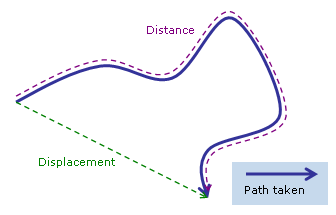
\includegraphics[scale=0.7]{Distancedisplacement}
            %     \fontfamily{cmss}\selectfont {
            %         \caption{Distance and displacement}
            %     }
            %     \label{fig:my_label}
            % \end{figure}
       
            
   		\item Cực trị tự do
            \begin{itemize}
                \item $f(x, y)$ đạt cực đại tương đối tại $M_{0}(x_{0}, y_{0})$ :  
                    \[f(x, y) = f(x_{0} + \Delta x, y_{0} + \Delta y) - f(x_{0}, y_{0}) \leqslant 0 \quad \forall (\Delta x, \Delta y) \to (0, 0)
                    \] 
                \item  $f(x, y)$ đạt cực tiểu tương đối tại $M_{0}(x_{0}, y_{0})$ :  
                \[f(x, y) = f(x_{0} + \Delta x, y_{0} + \Delta y) - f(x_{0}, y_{0}) \geqslant  0 \quad \forall (\Delta x, \Delta y) \to (0, 0)
                \] 
                \item $M_{0}$ là điểm tới hạn :
                    \[\dfrac{\partial f}{\partial x}(M_{0}) = \dfrac{\partial f}{\partial y}(M_{0}) = 0\]

                    hoặc một trong hai không tồn tại.
                \item Điều kiện cần :
                    Nếu hàm số có cực trị tại $M_{0}$ thì $M_{0}$ là điểm tới hạn.
                \item Điều kiện đủ :
                    Ta có điểm $M_{0}$ là điểm tới hạn của hàm số.

                    Để $M_{0}$ là điểm cực trị của hàm số:

                    Ta xét:
                        \[A = f''_{xx}(x_{0}, y_{0})\]
                        \[B = f''_{xy}(x_{0}, y_{0})\]
                        \[C = f''_{yy}(x_{0}, y_{0})\]
                    \indent Để $M_{0}$ là điểm cực trị của hàm số:
                        \[AC - B^{2} > 0\]
                    Nếu $A > 0$ hoặc $C > 0$ $\Rightarrow$ cực tiểu địa phương.

                    Nếu $A < 0$ hoặc $C < 0$ $\Rightarrow$ cực đại địa phương.
                    
                    Nếu $AC - B^{2} < 0$ $\Rightarrow$ không phải cực trị.

                    Nếu $AC - B^{2} = 0$ $\Rightarrow$ cũng có thể là có, cũng có thể là không.
            
            \end{itemize}
                
        \item Cực trị có điều kiện
            \begin{itemize}
                \item Nhân tử  Lagrange.
                    
                Xét tìm cực trị hàm số $f(x, y)$ với điều kiện $\varphi(x, y) = 0$
                \[L(x, y, \lambda) = f(x, y) + \lambda . \varphi(x, y)\]
                Ta có các điểm dừng:
                \begin{align*}
                L'_{x} &= 0 & f'_{x}(x, y) + \lambda.\varphi'_{x}(x, y) &= 0\\
                L'_{y} &= 0 & f'_{y}(x, y) + \lambda.\varphi'_{y}(x, y) &= 0 \\
                L'_{\lambda} & = 0 & \varphi(x, y) &= 0
            \end{align*}
                \[\Rightarrow \lambda, x_{0}, y_{0}\]
                \[\Rightarrow M(x_{0}, y_{0})\]
                Dựa vào dấu của $d^{2}L(M_{0})$ ta biết được $M_{0}(x_{0}, y_{0})$ có phải là điểm cực trị hay không.
                \[d^{2}L(M_{0}) = L''_{xx}(M_{0})dx^{2} + 2L''_{xy}(M_{0})dxdy + L''_{yy}(M_{0})dy^{2}\]

                Chú ý:
                \[d\varphi(M_{0}) = \varphi'_{x}(M_{0}) dx + \varphi'_{y}(M_{0}) dy\]
                \[\Rightarrow dy = -\dfrac{\varphi'_{x}(M_{0})dx}{\varphi'_{y}(M_{0})}\]
                Nếu $d^{2}L(M_{0}) > 0 \Rightarrow$ cực tiểu.
                
                Nếu $d^{2}L(M_{0}) < 0 \Rightarrow$ cực đại.
                
                Nếu không xác đinh thì không phải cực trị.
            \end{itemize}
        \item Tích phân bội 2
        
            
    \end{enumerate}
    
\end{center}




}
\end{document}